\documentclass{report}
\usepackage{graphicx} % Required for inserting images
\usepackage[italian]{babel}
\usepackage{tikz}
\usepackage{hyperref}
\usepackage{amsmath}
\usepackage{xcolor}
\usepackage{float}
\usepackage{soul}
\usepackage{listings} % Per evidenziare il codice

\definecolor{lightgray}{rgb}{0.9,0.9,0.9} % Definizione colore sfondo
\definecolor{darkgreen}{rgb}{0.0, 0.5, 0.0}

\lstset{
    backgroundcolor=\color{lightgray}, % Sfondo grigio
    basicstyle=\ttfamily, % Font monospaziato
    % frame=single, % Bordo attorno al codice
    tabsize=4, % Dimensione tabulazione
    breaklines=true, % Permette di andare a capo automaticamente
    numbers = left,
    numberstyle=\small\color{gray}
}

\title{\huge\textbf{{Modellazione e Analisi di Sistemi}}}
\date{}

\begin{document}

\maketitle

\tableofcontents
\newpage

\chapter{Abstract State Machines}

Le ASM sono delle FSM (\textit{Final State Machines}) con stati generalizzati; rappresentano la forma 
matematica di macchine che estendono la nozione di FSM, \textbf{ampliando la definzione di stato} 
e \textbf{modificando la forma delle transizioni}.

\subsubsection{Stati}
Gli stati di controllo non strutturati vengono sostituiti da stati (strutturati) che 
modellano:
\begin{itemize}
    \item \textbf{dati} complessi arbitrati (con domini di base e funzioni per la struttura)
    \item \textbf{operazioni} per la manipolazione di dati
\end{itemize}

\noindent Possiamo definire gli stati come delle \textit{algebre}.

\begin{figure}[H]
    \centering
    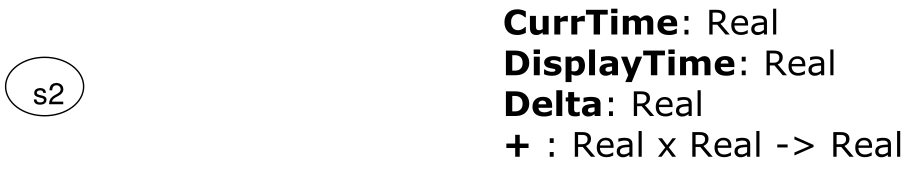
\includegraphics[width=0.8\linewidth]{chapters/1-asm/images/stati.png}
\end{figure}

\subsubsection{Transizioni}
Le transizione sono \textit{"regole"} che descrivono il cambiamento 
di funzioni da uno stato al successivo; permettono di modificare la 
struttura algebrica durante l'esecuzione della ASM.

\begin{center}
    \textit{if condition then Updates}
\end{center}

\noindent Negli FSM le transizioni sono rappresentate con delle frecce.

\newpage
Le ASM sono dotate di un ambiente di tool per:
\begin{itemize}
    \item editing
    \item simulazione
    \item validazione 
    \item verifica
    \item generazioni di casi di test
\end{itemize}

\noindent Un modello ASM può essere visto come pseudocodice su strutture dati astratte.

\subsubsection{Da FSM a ASM}
\begin{figure}[H]
    \centering
    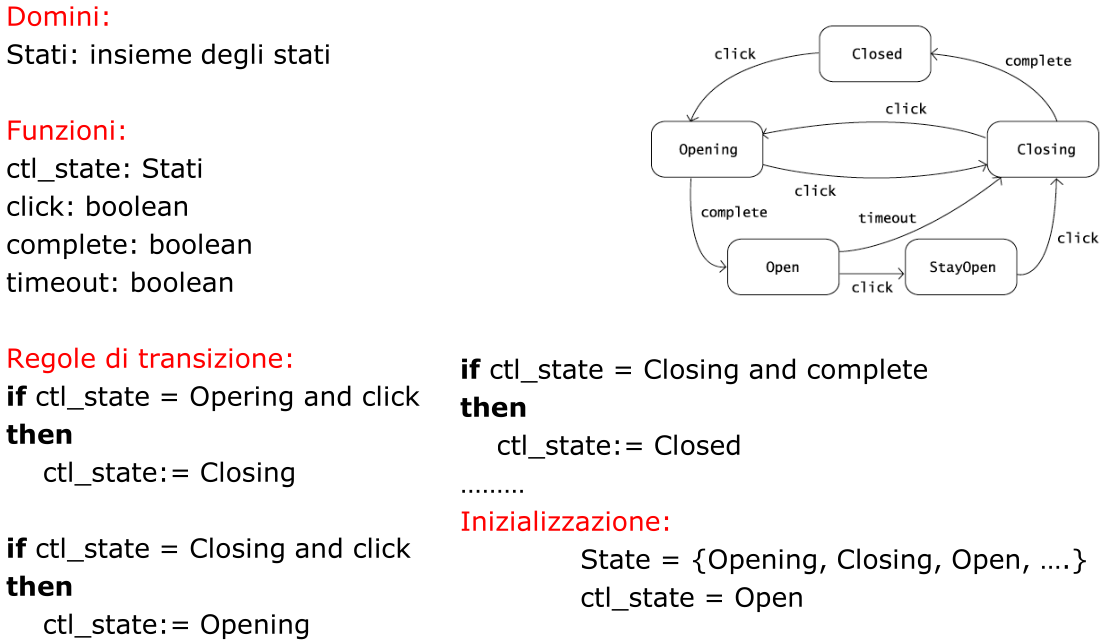
\includegraphics[width=0.92\linewidth]{chapters/1-asm/images/fsm-asm2.png}
\end{figure}

\noindent Possiamo definire ASM = (header, body, main rule, inizialization)

\begin{figure}[H]
    \centering
    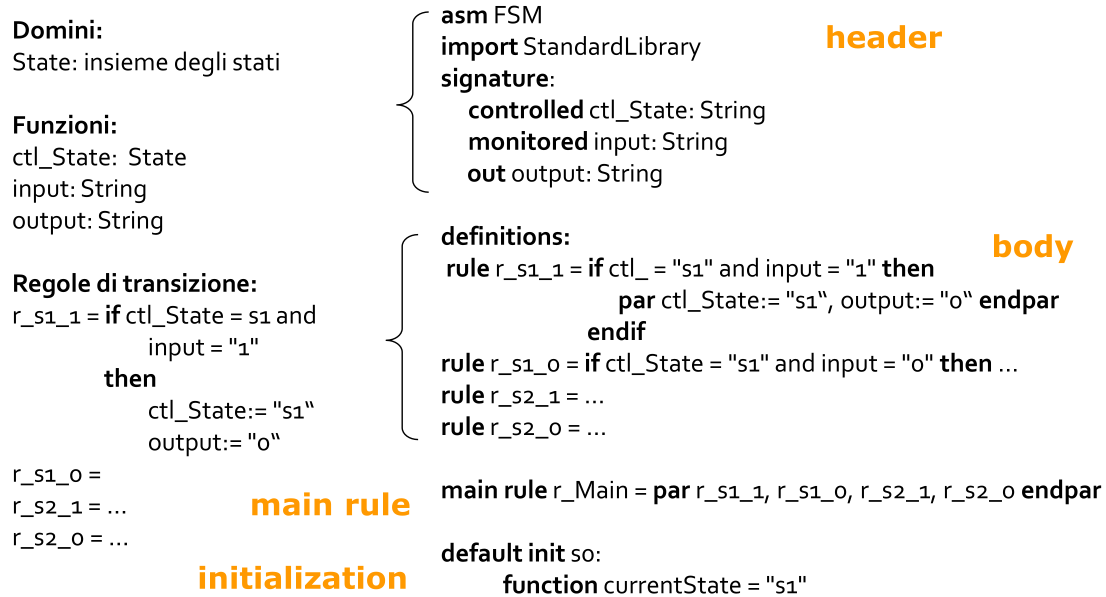
\includegraphics[width=0.92\linewidth]{chapters/1-asm/images/comp-asm.png}
\end{figure}

\section{Formalismo}

\subsection{Vocabolario}
\underline{\textbf{DEF:}} Un \textbf{vocabolario} $\Sigma$ è una collezione finita di nomi di 
funzioni.

\noindent Le funzioni possono essere dinamiche o statiche, a seconda che l'interpretazione 
del nome della funzione cambia o no da uno stato al successivo (funzioni 
in senso matematico).

\subsection{Costanti}
Le funzioni statiche di arietà zero sono dette \textbf{costanti}. Ogni 
vocabolario contiene sempre le costanti \textit{undef, true, false}.

\noindent Ad esempio:
\begin{itemize}
    \item i numeri sono costanti numeriche
    \item \texttt{voto = 30}
\end{itemize}


\subsection{Funzioni statiche}
Le funzioni statiche (arietà $>0$) sono definite tramite una legge fissa.

\noindent Ad esempio:
\begin{itemize}
    \item operazioni tra numeri (+, -, \dots)
    \item operazioni tra booleani (AND, OR, \dots)
    \item \texttt{max(m, n)}
\end{itemize}

\subsection{Fuzioni dinamiche}
Le funzioni dinamiche di arietà zero sono le variabili dei linguaggi 
di programmazione.

\subsection{Stato ASM}
\underline{\textbf{DEF:}} Fissato un vocabolario $\Sigma$, uno \textbf{stato} A del 
vocabolario $\Sigma$ è un insieme non vuoto $X$, detto \textit{superuniverso di A}, con 
le interpretazioni dei nomi delle funzioni di $\Sigma$.

\noindent Da questa definizione, segue che:
\begin{itemize}
    \item se $f$ è un nome di funzione \textit{n-aria} di $\Sigma$, allora 
    la sua interpretazione $f^A$ è una funzione da $X^n$ a $X$
    \item Se $c$ è un nome di costante di $\Sigma$, allora la sua interpretazione $c^A$ è un elemento di $X$
\end{itemize}

\noindent Possiamo definire il superuniverso come un \textit{"dominio di 
interpretazione"}; i simboli del vocabolario, presi singoralmente, sono soltanto simboli.

\subsection{Domini ASM}
Il superuniverso di uno stato ASM è suddiviso in \textit{universi}, 
rappresentati dalle loro funzioni caratteristiche.

\begin{center}
    \textit{Se A è un sottoinsieme dell'insieme X, la funzione caratteristica di A è quella 
    funzione da X all'insieme $\{0 , 1\}$ che sull'elemento x $\in$ X vale 1 se x appartiene ad A, e vale 0 in caso contrario.  }
\end{center}

\noindent Ogni universo rappresenta un dominio. In base a questa 
rappresentazione degli insiemi in termini di funzioni caratteristiche, uno stato di una 
ASM consente di modellare \textbf{domini eterogenei}.

\noindent Alcuni esempi di domini:
\begin{itemize}
    \item predefiniti, come \texttt{Interi, String, \dots}
    \item definiti dall'utente, come tipi astratti o a partire da altri domini
\end{itemize}

\subsubsection{Esempio}
Dominio $X=\{1,2,a,b,mario,pippo\}$, ripartito in domini:
\begin{itemize}
    \item $Interi = \{1.2\}$
    \item $Char = \{a,b\}$
    \item $String = \{mario, pippo\}$
\end{itemize}

\subsection{Termini ASM}
\underline{\textbf{DEF:}} i termini di $\Sigma$ sono espressioni sintattiche così costruite:
\begin{enumerate}
    \item Variabili $v_0, v_1, v_2, \dots$ sono termini 
    \item Costanti $c$ di $\Sigma$ sono termini 
    \item Se $f$ è un nome di funzione \textit{n-aria} di $\Sigma$ e 
    $t_1, \dots, t_n$ sono termini 
    
    $\Rightarrow f(t1, \dots, t_n)$ è un termine 
\end{enumerate}

\noindent Ad esempio:
\begin{itemize}
    \item $v_0 + v_1$
    \item $1 + (v_2 * 0)$
\end{itemize}

\noindent Un termine che non contiene variabili è detto chiuso. I termini 
sono \textit{oggetti sintattici}. \textbf{Assumono significato (o semantica)
nello stato}; il suo valore è l'\textit{interpretazione del termine} in $A$.



\chapter{Prime tecniche di analisi}
\section{Analisi di un modello}
Per l'analisi di un modello si usano due approcci:
\begin{itemize}
    \item \textbf{Validazione:} necessaria per controllare che il
    sistema soddisfi i requisiti richiesti
    \item \textbf{Verifica:} necessaria per garantire proprietà
    (safety, leaveness, assenza deadlock,
    reachability, ecc.)
\end{itemize}
La validazione dovrebbe precedere la verifica per individuare errori il prima possibile
e evitare di provare proprietà corrette su specifiche incorrette.

\noindent Sono possibili due prime forme di analisi
sul ground model:
\begin{itemize}
    \item Garanzia degli invarianti
    \item Validazione tramite scenari
\end{itemize}

\subsection{Garanzia degli invarianti}
In un modello ASM gli \textit{invarianti} sono usati per esprimere \textbf{vincoli} su funzioni e/o regole
che devono essere garantiti in ogni stato. 

\noindent In programmi AsmetaL usare gli invarianti è utile per scoprire errori di modellazione
In generale, l'assenza di violazione di invarianti non può essere considerata una prova della correttezza del modello, mentre la violazione di
assiomi, è prova della incorrettezza del modello

\noindent Dochiarazione degli invarianti:
\begin{itemize}
    \item Gli invarianti vanno dichiarati subito prima della main rule
    \item Ogni invariante è dichiarato mediante la keyword \textit{invariant} che precede il nome attribuito all'assioma
    \item Le funzioni e regole su cui è espresso il vincolo vanno listate dopo la keyword \textit{over}
\end{itemize}

\begin{figure}[H]
    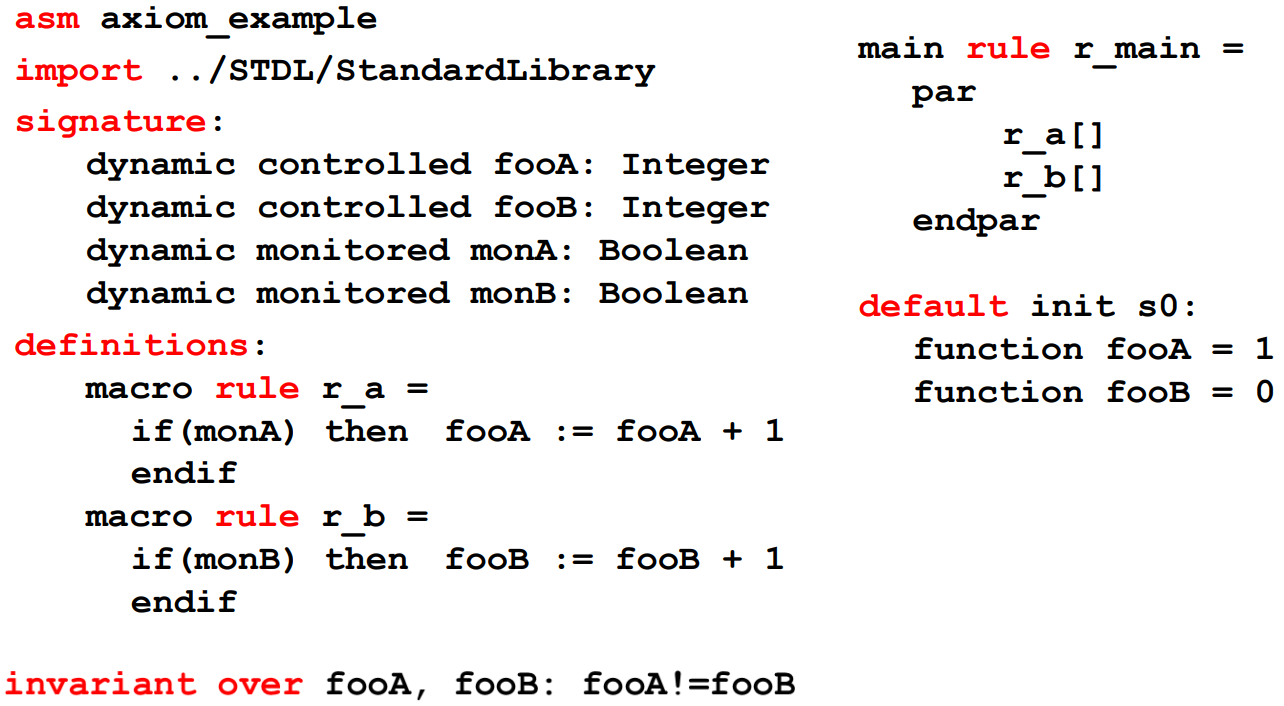
\includegraphics[width=0.8\linewidth]{chapters/2/images/axiomex.png}
\end{figure}


\subsection{Validazione tramite scenari}
\begin{itemize}
    \item \textbf{Tecniche:} Generazione di scenari, sviluppo di prototipi, animazione, simulazione, testing 
    \item \textbf{Scenario:} descrizione di un possibile comportamento del sistema (interazione osservabile tra il sistema ed il suo
    ambiente in specifiche situazioni)
\end{itemize}

\noindent Gli scenari sono costituiti attraverso una notazione testuale (Avalla)
Semantica chiara (definita in termini di ASM) e capacità di descrivere anche dettagli interni (non solo black box come per UML use cases, ma
anche informazioni sullo stato).

\subsubsection{Da attore UML  a attore ASM}
\noindent Nell'UML use case l'attore interagisce col sistema, uno o più scenari possono essere generati per
ogni caso d'uso, però visione BLACK BOX.
\noindent L'ASM Observer può verificare lo stato interno della macchina e gli invarianti, e
richiede l'esecuzione di regole arbitrarie.

\begin{figure}[H]
    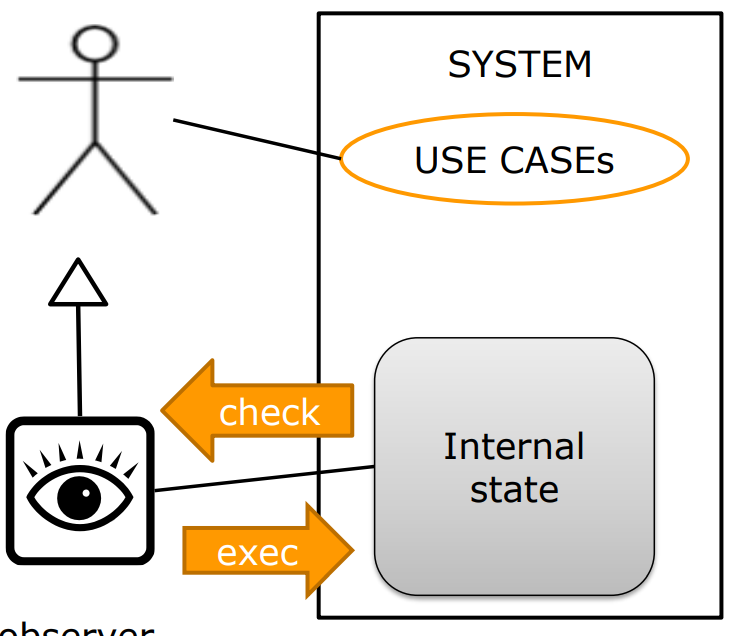
\includegraphics[width=0.5\linewidth]{chapters/2/images/attoreASM.png}
\end{figure}

\subsubsection{Doppio uso degli scenari}
\begin{itemize}
    \item Due tipi di attori esterni:
    \item \begin{itemize}
        \item \textbf{User:} ha una visione \textit{black box} del sistema
        \item \textbf{Observer:} ha una visione \textit{grey box}
    \item Due obiettivi per gli scenari:
    \item \begin{itemize}
        \item \textbf{Validazione classica:} azione dell'utente e reazioni della macchina
        \item \textbf{Attività di testing:} ispezione dell’observer dello stato interno
        della macchina
    \end{itemize}
    \end{itemize}
\end{itemize}

\subsubsection{Scenario ASM}
Sequenza di interazione consentite delle azioni:
\begin{itemize}
    \item da parte di user/observer: 
    \begin{itemize}
        \item \textbf{set} the environment (i.e. the values of
        monitored/shared functions)
        \item \textbf{check} for the machine outputs (i.e. the values of
        out functions)
        \item \textbf{check} the machine state and invariants
        \item \textbf{ask} for the execution of given transition rules
    \end{itemize}
    \item da parte della macchina: 
    \textbf{makes} one \textit{step} as reaction of the actor actions
\end{itemize}

\subsubsection{Primitive di AvValLa - Asm Validation Language}
\begin{figure}[H]
    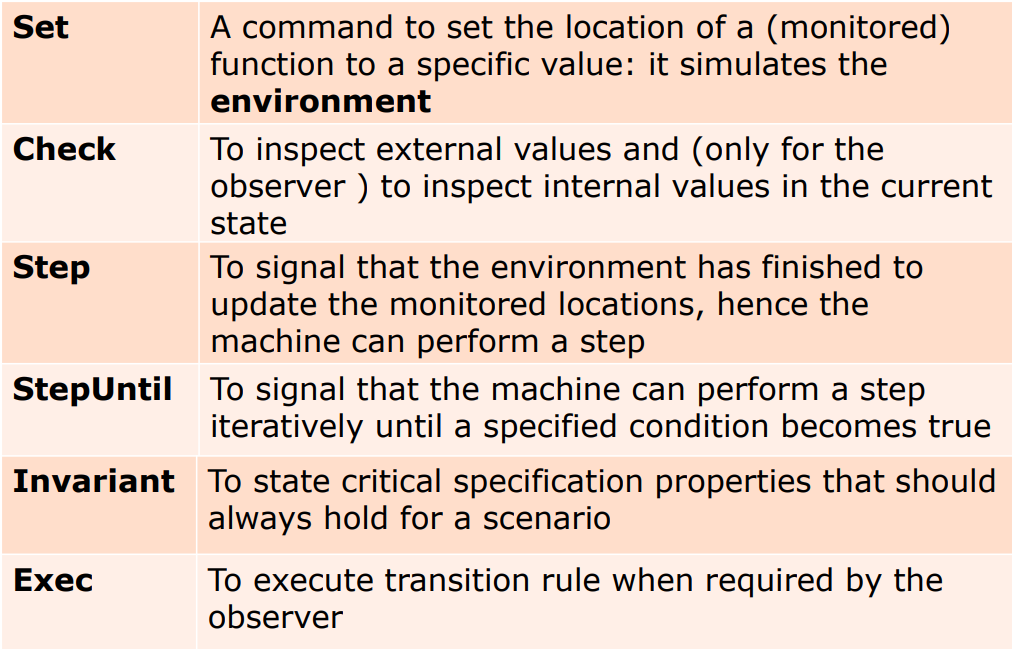
\includegraphics[width=0.8\linewidth]{chapters/2/images/Avalla.png}
\end{figure}

\subsubsection{Sintassi Avalla}
\begin{figure}[H]
    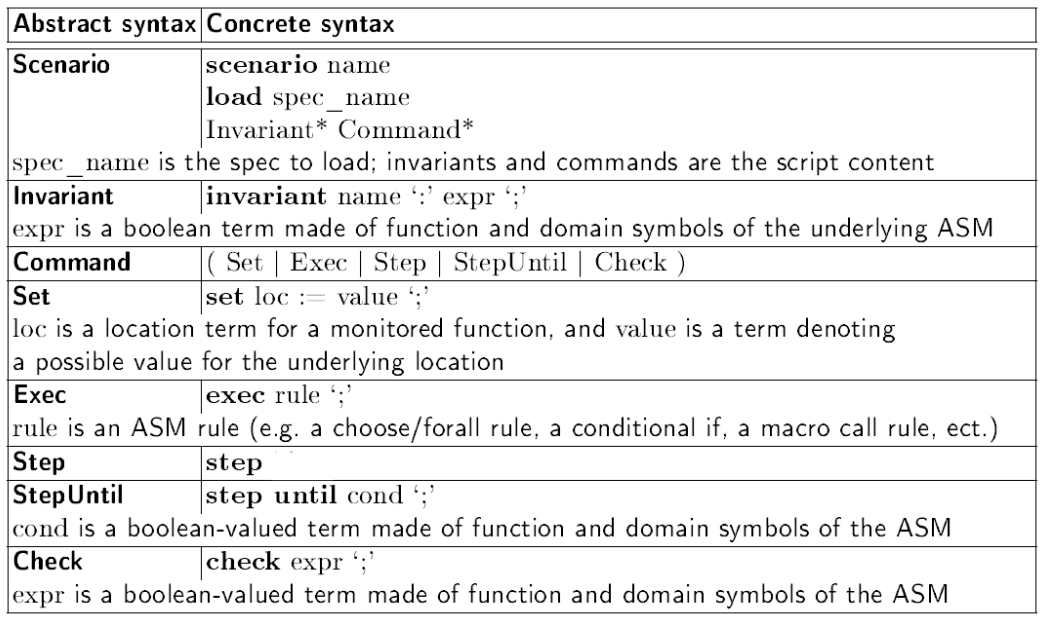
\includegraphics[width=0.8\linewidth]{chapters/2/images/sintassiAvalla.png}
\end{figure}





\end{document}